\let\negmedspace\undefined
\let\negthickspace\undefined
\documentclass[journal,12pt,onecolumn]{IEEEtran}
\usepackage{cite}
\usepackage{amsmath,amssymb,amsfonts,amsthm}
\usepackage{algorithmic}
\usepackage{tasks}
\settasks{label=\brak{\Alph*}, label-width=3ex, item-indent=0pt, column-sep=2em}
\usepackage{graphicx}
\graphicspath{{./figs/}}
\usepackage{textcomp}
\usepackage{xcolor}
\usepackage{txfonts}
\usepackage{listings}
\usepackage{enumitem}
\usepackage{mathtools}
\usepackage{gensymb}
\usepackage{comment}
\usepackage{caption}
\usepackage[breaklinks=true]{hyperref}
\usepackage{tkz-euclide} 
\usepackage{listings}
\usepackage{gvv}                                        
%\def\inputGnumericTable{}                                 
\usepackage[latin1]{inputenc}     
\usepackage{xparse}
\usepackage{color}                  
                           
\usepackage{array}                                            
\usepackage{longtable}                              
          
\usepackage{calc}                                             
\usepackage{multirow}
\usepackage{multicol}
\usepackage{hhline}                                           
\usepackage{ifthen}   
                                         
\usepackage{lscape}
\usepackage{tabularx}
\usepackage{array}
\usepackage{float}
\usepackage{mhchem}
\newtheorem{theorem}{Theorem}[section]
\newtheorem{problem}{Problem}
\newtheorem{proposition}{Proposition}[section]
\newtheorem{lemma}{Lemma}[section]
\newtheorem{corollary}[theorem]{Corollary}
\newtheorem{example}{Example}[section]
\newtheorem{definition}[problem]{Definition}
\newcommand{\BEQA}{\begin{eqnarray}}
\newcommand{\EEQA}{\end{eqnarray}}
\newcommand{\define}{\stackrel{\triangle}{=}}
\theoremstyle{remark}
\newtheorem{rem}{Remark}

\begin{document}
\title{
ASSIGNMENT 1: GATE 2009 \\
CY: CHEMISTRY}
\author{EE25BTECH11039 - Manupati Manideep}
\maketitle
\renewcommand{\thefigure}{\theenumi}
\renewcommand{\thetable}{\theenumi}
\begin{enumerate}

\item The $^{31}P$ NMR spectrum of $P_4S_3$ consists of
    \begin{enumerate}
        \begin{multicols}{2}
        \item a singlet
        \item a doublet and a triplet
        \item 
 a doublet and a quartet
        \item two doublets
        \end{multicols}
      \hfill{\brak{\text{GATE CY-2009}}}
    \end{enumerate}



\item The geometry around the central atom in $ClF_4^+$ is
    \begin{enumerate}
        \begin{multicols}{4}
        \item square planar
        \item square pyramidal
        \item octahedral
        \item trigonal bipyramidal
       
  \end{multicols}
        \hfill{\brak{\text{GATE CY-2009}}}
    \end{enumerate}



\item The correct statement about the Cu-N bond distances in $\sbrak{Cu\brak{NH_3}_6}^{2+}$ is
    \begin{enumerate}
        \item all the bond distances are equal
        \item the axial bonds are longer than the equatorial ones
        \item the equatorial bonds are longer than the axial ones
        \item all the bond distances are unequal
        \hfill{\brak{\text{GATE 
 CY-2009}}}
    \end{enumerate}



\item The reaction of phosgene with an excess of $NH_3$ produces
    \begin{enumerate}
        \item $HN=C=O$
        \item $H_2N-C\brak{Cl}=O$
        \item $\brak{H_2N}_2C=O$
        \item $\brak{H_2N}_2CCl_2$
        \hfill{\brak{\text{GATE CY-2009}}}
    \end{enumerate}



\item The number of metal-metal bonds in $\sbrak{\brak{C_5H_5}Fe\brak{CO}}_2$ is
    \begin{enumerate}
        \begin{multicols}{4}
        \item zero
    
     \item one
        \item two
        \item three
        \end{multicols}
        \hfill{\brak{\text{GATE CY-2009}}}
    \end{enumerate}



\item The coordination number of the $Ba^{2+}$ ions in barium fluoride is 8. The coordination number of the fluoride ion is
    \begin{enumerate}
        \begin{multicols}{4}
        \item 8
        \item 4
      
   \item 1
        \item 2
        \end{multicols}
        \hfill{\brak{\text{GATE CY-2009}}}
    \end{enumerate}



\item In the transformation of oxyhaemoglobin to deoxyhaemoglobin
    \begin{enumerate}
        \item $Fe^{2+}$ in the low spin state changes to $Fe^{2+}$ in the high spin state
        \item $Fe^{2+}$ in the low spin state changes to $Fe^{3+}$ in the low spin state
        \item $Fe^{2+}$ in the 
 high spin state changes to $Fe^{2+}$ in the low spin state
        \item $Fe^{2+}$ in the high spin state changes to $Fe^{3+}$ in the high spin state
        \hfill{\brak{\text{GATE CY-2009}}}
    \end{enumerate}



\item For the compound
    \begin{figure}[H]
        \centering
        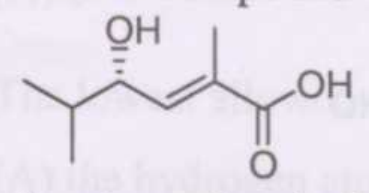
\includegraphics[width=0.4\columnwidth]{q8}
        \caption*{}
        \label{fig:q8}
    \end{figure}
    the stereochemical notations are
    \begin{enumerate}
 
        \begin{multicols}{4}
        \item 2Z, 4R
        \item 2Z, 4S
        \item 2E, 4R
        \item 2E, 4S
        \end{multicols}
        \hfill{\brak{\text{GATE CY-2009}}}
    \end{enumerate}



\item The compound
    \begin{figure}[H]
        \centering
        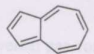
\includegraphics[width=0.3\columnwidth]{q9}
        \caption*{}
  
       \label{fig:q9}
    \end{figure}
    is
    \begin{enumerate}
        \item aromatic and has high dipole moment
        \item aromatic and has no dipole moment
        \item non-aromatic and has high dipole moment
        \item anti-aromatic and has no dipole moment
        \hfill{\brak{\text{GATE CY-2009}}}
    \end{enumerate}



\item In the reaction

\begin{center}
    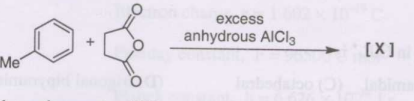
\includegraphics[width=0.5\columnwidth]{q10}
\end{center}

the major product X is

\begin{enumerate}

\begin{multicols}{2} 
 
     \item 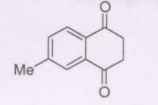
\includegraphics[width=0.25\columnwidth]{q10a}
    \item 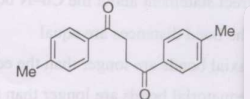
\includegraphics[width=0.25\columnwidth]{q10b}
    \item 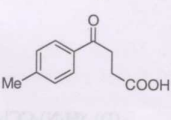
\includegraphics[width=0.25\columnwidth]{q10c}
    \item 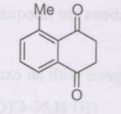
\includegraphics[width=0.25\columnwidth]{q10d}
   
\end{multicols}

\end{enumerate}
\hfill{\brak{\text{GATE CY-2009}}}



\item In the reaction

\begin{center}
    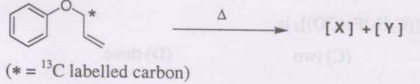
\includegraphics[width=0.7\columnwidth]{q11}
\end{center}

the major products X and Y are

\begin{enumerate}

\begin{multicols}{2}
    \item 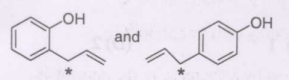
\includegraphics[width=0.25\columnwidth]{q11a}
    \item 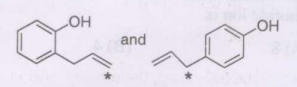
\includegraphics[width=0.25\columnwidth]{q11b}
    \item 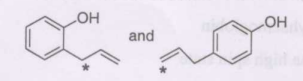
\includegraphics[width=0.25\columnwidth]{q11c}
    \item 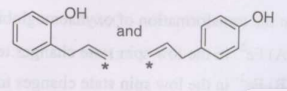
\includegraphics[width=0.25\columnwidth]{q11d}
\end{multicols}
\hfill{\brak{\text{GATE CY-2009}}}

\end{enumerate}



\item In the reaction
    \begin{center}
        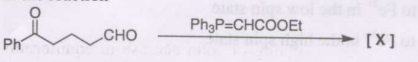
\includegraphics[width=0.7\columnwidth]{q12}
      
    \end{center}
    the major product X is
    \begin{enumerate}
    \begin{multicols}{2}
  
   \item 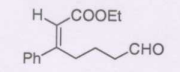
\includegraphics[width=0.4\columnwidth]{figs/q12a.png}
    \item 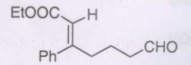
\includegraphics[width=0.4\columnwidth]{figs/q12b.png}
    \item 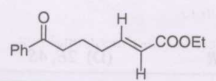
\includegraphics[width=0.4\columnwidth]{figs/q12c.png}
    \item 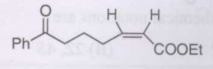
\includegraphics[width=0.4\columnwidth]{figs/q12d.png}
\end{multicols}
\end{enumerate}
\hfill{\brak{\text{GATE CY-2009}}}




\item The most suitable reagent combination to bring out the following transformation
    \begin{figure}[H]
        \centering
        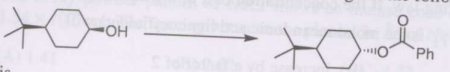
\includegraphics[width=0.7\columnwidth]{q13}
        \caption*{}
        \label{fig:q13}
    \end{figure}
    is
    \begin{enumerate}
        \begin{multicols}{2}
        \item PhCOCl and pyridine
   
         \item DCC and PhCOOH
        \item PhBr, CO and $Pd\brak{PPh_3}_4$
        \item EtOOC-N=N-COOEt, $PPh_3$ and PhCOOH
        \end{multicols}
        \hfill{\brak{\text{GATE CY-2009}}}
    \end{enumerate}



\item In the two steps reaction sequence
    \begin{figure}[H]
        \centering
        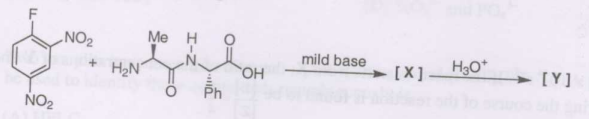
\includegraphics[width=0.8\columnwidth]{q14}
        \caption*{}
        \label{fig:q14}
    \end{figure}
 
    the major product Y is
    \begin{enumerate}
        
   \begin{multicols}{2}
         \item 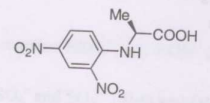
\includegraphics[width=0.25\columnwidth]{figs/q14a.png}
         \item 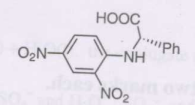
\includegraphics[width=0.25\columnwidth]{figs/q14b.png}
         \item  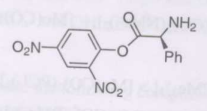
\includegraphics[width=0.25\columnwidth]{figs/q14c.png}
         \item 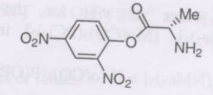
\includegraphics[width=0.25\columnwidth]{figs/q14d.png}
\end{multicols}

\end{enumerate}
\hfill{\brak{\text{GATE CY-2009}}}



\item Among the following, the system that would require the least amount of thermal energy to bring its temperature to 80$\degree$C is
    \begin{enumerate}
        \begin{multicols}{2}
   
         \item 200 g of water at $40\degree C$
        \item 100 g of water at $20\degree C$
        \item 150 g of water at $50\degree C$
        \item 300 g of water at $30\degree C$
        \end{multicols}
        \hfill{\brak{\text{GATE CY-2009}}}
    \end{enumerate}



\item Among the following, the reaction that is accompanied by a decrease in the entropy is
    \begin{enumerate}
   
         \item $N_2\brak{g} + 3H_2\brak{g} \rightarrow 2NH_3\brak{g}$
        \item $C_6H_{12}O_6\brak{s} + 6O_2\brak{g} \rightarrow 6CO_2\brak{g} + 6H_2O\brak{l}$
        \item $PCl_5\brak{s} \rightarrow PCl_3\brak{l} + Cl_2\brak{g}$
        \item $2H_2O\brak{l} \rightarrow 2H_2\brak{g} + O_2\brak{g}$
        \hfill{\brak{\text{GATE CY-2009}}}
    \end{enumerate}



\item The number of degrees of freedom of a system consisting of solid sucrose in equilibrium with an aqueous solution of sucrose is
    \begin{enumerate}
        \begin{multicols}{4}
  
         \item 0
        \item 1
        \item 2
        \item 3
        \end{multicols}
        \hfill{\brak{\text{GATE CY-2009}}}
    \end{enumerate}



\item The lowest allowed energy is equal to zero for
    \begin{enumerate}
        \begin{multicols}{2}
        \item the hydrogen atom
        \item a rigid rotor
  
         \item a harmonic oscillator
        \item a particle in a 3-dimensional box
        \end{multicols}
        \hfill{\brak{\text{GATE CY-2009}}}
    \end{enumerate}



\item According to the Debye-Hückel limiting law, if the concentration of a dilute aqueous solution of KCl is increased 4-fold, the value of $\ln \gamma_{\pm}$ \brak{\gamma_{\pm}\text{ is the molal mean ionic activity coefficient}} will
    \begin{enumerate}
        \begin{multicols}{2}
        \item decrease by 
 a factor of 2
        \item increase by a factor of 2
        \item decrease by a factor of 4
        \item increase by a factor of 4
        \end{multicols}
        \hfill{\brak{\text{GATE CY-2009}}}
    \end{enumerate}



\item For the parallel first order reaction shown below
\begin{align*}
     &X \xrightarrow{k_1} Y\\
     &X \xrightarrow{k_2} Z
\end{align*}
    the value of $k_1$ is $1 
 \times 10^{-4} s^{-1}$. If the reaction starts from X, the ratio of the concentrations of Y and Z at any given time during the course of the reaction is found to be $\frac{\sbrak{Y}}{\sbrak{Z}} = \frac{1}{4}$.
 The value of $k_2$ is
    \begin{enumerate}
        \begin{multicols}{2}
        \item $1 \times 10^{-4} s^{-1}$
        \item $2.5 \times 10^{-5} s^{-1}$
        \item $4 \times 10^{-4} s^{-1}$
        \item $4 \times 10^{4} s^{-1}$
        \end{multicols}
        \hfill{\brak{\text{GATE CY-2009}}}
    \end{enumerate}
  \end{enumerate}  
  \vspace{1.5cm}
\begin{center}
\section*{Q.21 - Q. 60 carry two marks each.}

\end{center}

\begin{enumerate}[resume]
\item The 
 correct order of $\nu_{\mathrm{CO}}$ for the compounds 
$\mathrm{\sbrak{Mo\brak{CO}_3\brak{NMe_3}_3}}$, 
$\mathrm{\sbrak{Mo\brak{CO}_3\brak{POPh_3}_3}}$, 
$\mathrm{\sbrak{Mo\brak{CO}_3\brak{PMe_3}_3}}$, 
$\mathrm{\sbrak{Mo\brak{CO}_3\brak{PCPh_3}_3}}$ in the IR spectrum is 

\begin{enumerate}
\item $\mathrm{\sbrak{Mo\brak{CO}_3\brak{NMe_3}_3}} > \mathrm{\sbrak{Mo\brak{CO}_3\brak{POPh_3}_3}} > \mathrm{\sbrak{Mo\brak{CO}_3\brak{PMe_3}_3}} > \mathrm{\sbrak{Mo\brak{CO}_3\brak{PCPh_3}_3}}$
\item $\mathrm{\sbrak{Mo\brak{CO}_3\brak{PCPh_3}_3}} > \mathrm{\sbrak{Mo\brak{CO}_3\brak{PMe_3}_3}} > \mathrm{\sbrak{Mo\brak{CO}_3\brak{POPh_3}_3}} > \mathrm{\sbrak{Mo\brak{CO}_3\brak{NMe_3}_3}}$
\item $\mathrm{\sbrak{Mo\brak{CO}_3\brak{PMe_3}_3}} > \mathrm{\sbrak{Mo\brak{CO}_3\brak{NMe_3}_3}} > \mathrm{\sbrak{Mo\brak{CO}_3\brak{PCPh_3}_3}} > \mathrm{\sbrak{Mo\brak{CO}_3\brak{POPh_3}_3}}$
\item $\mathrm{\sbrak{Mo\brak{CO}_3\brak{POPh_3}_3}} > \mathrm{\sbrak{Mo\brak{CO}_3\brak{PMe_3}_3}} > \mathrm{\sbrak{Mo\brak{CO}_3\brak{NMe_3}_3}} > \mathrm{\sbrak{Mo\brak{CO}_3\brak{PCPh_3}_3}}$

\hfill{\brak{\text{GATE CY-2009}}}
\end{enumerate}



 
\item 2.5 g of an iron compound upon suitable treatment yielded 0.391 g of iron\brak{III} oxide.
 The percentage of iron in the compound is \brak{atomic weight of Fe: 55.847, O: 15.994}
    \begin{enumerate}
        \begin{multicols}{4}
        \item 10.94
        \item 12.15
        \item 11.31
        \item 9.11
        \end{multicols}
        \hfill{\brak{\text{GATE CY-2009}}}
    \end{enumerate}



\item In the reaction
    \begin{align*}
     Ph_3P \xrightarrow{MeI} \sbrak{X} \xrightarrow{n-BuLi} \sbrak{Y}
    \end{align*}
    
 the compounds X and Y, respectively, are
    \begin{enumerate}
        \item $\sbrak{Ph_3P\brak{Me}I}$;
 $Ph_3P=CH-CH_2-CH_2-CH_3$
        \item $\sbrak{Ph_3P\brak{Me}}\sbrak{I}$; $Ph_3P=CH_2$
        \item $\sbrak{Ph_3P\brak{Me}_2}$;
 $Ph_3P=CH_2$
        \item $\sbrak{Ph_3P\brak{Me}}\sbrak{I}$;
 $Ph_3P$
        \hfill{\brak{\text{GATE CY-2009}}}
    \end{enumerate}



\item The $^1$H NMR spectrum of HD consists of a
    \begin{enumerate}
        \begin{multicols}{2}
        \item singlet
        \item 1:1 doublet
        \item 1:1:1 triplet
        \item 1:2:1 triplet
        \end{multicols}
        \hfill{\brak{\text{GATE CY-2009}}}
    \end{enumerate}



\item The X-ray powder pattern of 
 NaCl shows an intense cone at $\theta = 15.87\degree$ using X-rays of wavelength $1.54 \times 10^{-8}$ cm.
 The spacing between the planes \brak{in \AA} of NaCl crystal is
    \begin{enumerate}
        \begin{multicols}{4}
        \item 1.41
        \item 2.82
        \item 4.23
        \item 5.63
        \end{multicols}
        \hfill{\brak{\text{GATE CY-2009}}}
    \end{enumerate}



\item Among the following, the isoelectronic and isostructural pair is
    \begin{enumerate}
        
 \begin{multicols}{2}
        \item $CO_2$ and $SO_2$
        \item $SO_3$ and $SeO_3$
        \item $NO_2^+$ and $TeO_2$
        \item $SiO_4^{4-}$ and $PO_4^{3-}$
        \end{multicols}
        \hfill{\brak{\text{GATE CY-2009}}}
    \end{enumerate}



\item Two samples have been given to you: $\sbrak{NiCl_2\brak{PPh_3}_2}$ and $\sbrak{PdCl_2\brak{PPh_3}_2}$.
 A physical method that can be used to identify these compounds unambiguously is
    \begin{enumerate}
        \begin{multicols}{2}
        \item HPLC
        \item magnetic susceptibility
        \item $^{13}C$ NMR spectroscopy
        \item Mössbauer spectroscopy
        \end{multicols}
        \hfill{\brak{\text{GATE CY-2009}}}
    \end{enumerate}



\item In the reaction $HSO_4^{-}\brak{aq} + OH^{-}\brak{aq} \Leftrightarrow SO_4^{2-}\brak{aq} + H_2O\brak{l}$, the conjugate acid-base pairs 
 are
    \begin{enumerate}
        \item $HSO_4^{-}$ and $SO_4^{2-}$;
 $H_2O$ and $OH^{-}$
        \item $HSO_4^{-}$ and $H_3O+$;
 $SO_4^{2-}$ and $OH^{-}$
        \item $HSO_4^{-}$ and $OH^{-}$;
 $SO_4^{2-}$ and $H_2O$
        \item $HSO_4^{-}$ and $OH^{-}$;
 $SO_4^{2-}$ and $H_3O^+$
        \hfill{\brak{\text{GATE CY-2009}}}
    \end{enumerate}



\item Designate the following complexes X, Y and Z as inert or labile: \\
    $X = \sbrak{Al\brak{C_2O_4}_3}^{3-}$, $Y = \sbrak{V\brak{H_2O}_6}^{2+}$, $Z = \sbrak{Cr\brak{C_2O_4}_3}^{3-}$
    \begin{enumerate}
        \item X and Y are inert;
 Z is labile
        \item X and Z are labile;
 Y is inert
        \item X is inert;
 Y and Z are labile
        \item X is labile;
 Y and Z are inert
        \hfill{\brak{\text{GATE CY-2009}}}
    \end{enumerate}



\item In the reaction sequence
    \begin{figure}[H]
        \centering
        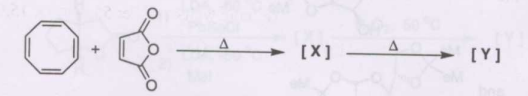
\includegraphics{q30}
        \caption*{}
        \label{fig:q30}
    \end{figure}
    X and Y, respectively, are

    \begin{enumerate}
   \begin{multicols}{2} 
    \item 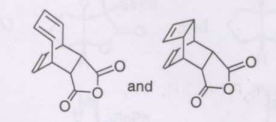
\includegraphics[width=0.25\columnwidth]{figs/q30a.png}
    \item 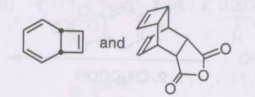
\includegraphics[width=0.25\columnwidth]{figs/q30b.png}
    \item 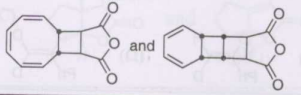
\includegraphics[width=0.25\columnwidth]{figs/q30c.png}
    \item 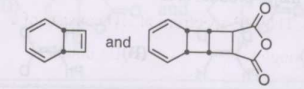
\includegraphics[width=0.25\columnwidth]{figs/q30d.png}
\end{multicols}
\end{enumerate}
\hfill{\brak{\text{GATE CY-2009}}}



\item The 
 major product X \brak{\text{based on the preferred conformation}} in the reaction
    \begin{center}
        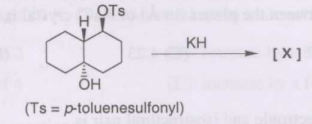
\includegraphics[width=0.5\columnwidth]{q31}
    \end{center}
    is
    \begin{enumerate}
   \begin{multicols}{2} 
    \item 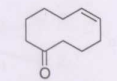
\includegraphics[width=0.25\columnwidth]{figs/q31a.png}
    \item 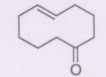
\includegraphics[width=0.25\columnwidth]{figs/q31b.png}
    \item 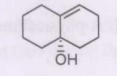
\includegraphics[width=0.25\columnwidth]{figs/q31c.png}
    \item 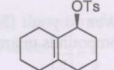
\includegraphics[width=0.25\columnwidth]{figs/q31d.png}
\end{multicols}
\end{enumerate}
\hfill{\brak{\text{GATE CY-2009}}}



\item In the reactions
    \begin{figure}[H]
        \centering
        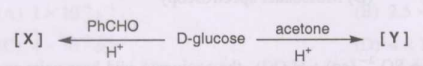
\includegraphics[width=0.8\columnwidth]{q32}
        \caption*{}
        \label{fig:q32}
  
   \end{figure}
    the major products X and Y, respectively, are
    \begin{enumerate}
    \begin{multicols}{2}
    \item 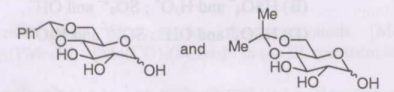
\includegraphics[width=0.4\columnwidth]{figs/q32a.png}
    \item 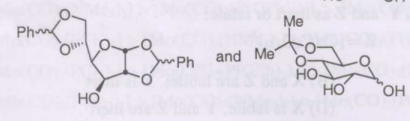
\includegraphics[width=0.4\columnwidth]{figs/q32b.png}
    \item 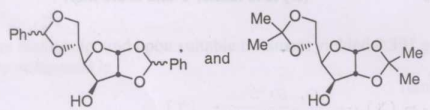
\includegraphics[width=0.4\columnwidth]{figs/q32c.png}
    \item 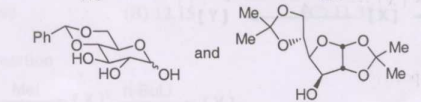
\includegraphics[width=0.4\columnwidth]{figs/q32d.png}
\end{multicols}
\end{enumerate}
\hfill{\brak{\text{GATE CY-2009}}}



\item In the reaction
    \begin{center}
        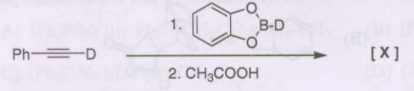
\includegraphics[width=0.7\columnwidth]{q33}
    \end{center}
    the major product X is
    \begin{enumerate}
   \begin{multicols}{2} 
    \item 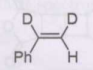
\includegraphics[width=0.25\columnwidth]{figs/q33a.png}
    \item 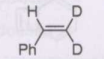
\includegraphics[width=0.25\columnwidth]{figs/q33b.png}
    \item 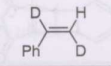
\includegraphics[width=0.25\columnwidth]{figs/q33c.png}
    \item 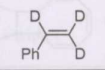
\includegraphics[width=0.25\columnwidth]{figs/q33d.png}
\end{multicols}
\end{enumerate}
\hfill{\brak{\text{GATE CY-2009}}}



\item Reaction 
 of m-methylanisole with lithium in liquid ammonia and t-butyl alcohol at $-33\degree$C generates compound X as the major product.
 Treatment of the compound X with dilute sulphuric acid produces compound Y as the major product.
 The compounds X and Y, respectively, are
\begin{enumerate}
   \begin{multicols}{2} 
    \item 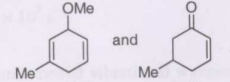
\includegraphics[width=0.25\columnwidth]{figs/q34a.png}
    \item 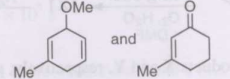
\includegraphics[width=0.25\columnwidth]{figs/q34b.png}
    \item 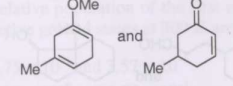
\includegraphics[width=0.25\columnwidth]{figs/q34c.png}
    \item 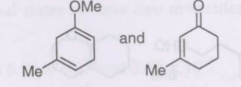
\includegraphics[width=0.25\columnwidth]{figs/q34d.png}
\end{multicols}
\end{enumerate}
\hfill{\brak{\text{GATE CY-2009}}}



\item The number of signals that appear in the broad-band decoupled $^{13}$C NMR spectrum of ortho-, meta- and para-dichlorobenzenes, respectively, are
    \begin{enumerate}
        \begin{multicols}{4}
        \item 3, 4 and 2
        \item 3, 3 and 2
        \item 4, 4 and 2
 
        \item 3, 4 and 4
        \end{multicols}
        \hfill{\brak{\text{GATE CY-2009}}}
    \end{enumerate}



\item In the reaction sequence
    \begin{center}
        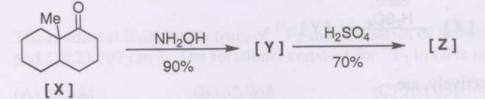
\includegraphics[width=0.8\columnwidth]{q36}
    \end{center}
    the structure of the major product Z and the overall yield for its formation from the ketone X, are
    \begin{enumerate}
   \begin{multicols}{2}
    \item 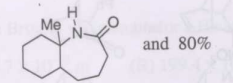
\includegraphics[width=0.25\columnwidth]{figs/q36a.png}
    \item 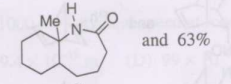
\includegraphics[width=0.25\columnwidth]{figs/q36b.png}
    \item \includegraphics[width=0.25\columnwidth]{figs/q36c.png}
    
 \item \includegraphics[width=0.25\columnwidth]{figs/q36d.png}
\end{multicols}
\end{enumerate}
\hfill{\brak{\text{GATE CY-2009}}}



\item In the reaction sequence
    \begin{figure}[H]
        \centering
        \includegraphics[width=0.8\columnwidth]{q37}
        \caption*{}
        \label{fig:q37}
    \end{figure}
    the major products X and Y, respectively, are
    \begin{enumerate}
    \begin{multicols}{2}
    \item \includegraphics[width=0.3\columnwidth]{figs/q37a.png}
    \item \includegraphics[width=0.3\columnwidth]{figs/q37b.png}
    \item \includegraphics[width=0.3\columnwidth]{figs/q37c.png}
    \item \includegraphics[width=0.3\columnwidth]{figs/q37d.png}
\end{multicols}
\end{enumerate}
\hfill{\brak{\text{GATE CY-2009}}}



\item In the reaction sequence
    \begin{figure}[H]
      
   \centering
        \includegraphics[width=0.6\columnwidth]{q38}
        \caption*{}
        \label{fig:q38}
    \end{figure}
    the major products X and Y, respectively, are
    \begin{enumerate}
 \begin{multicols}{2} 
    \item \includegraphics[width=0.3\columnwidth]{figs/q38a.png}
    \item \includegraphics[width=0.3\columnwidth]{figs/q38b.png}
    \item \includegraphics[width=0.3\columnwidth]{figs/q38c.png}
    \item \includegraphics[width=0.3\columnwidth]{figs/q38d.png}
\end{multicols}
\end{enumerate}
\hfill{\brak{\text{GATE CY-2009}}}



\item In the reaction sequence
    \begin{figure}[H]
        \centering
        \includegraphics[width=0.8\columnwidth]{q39}
        
 \caption*{}
        \label{fig:q39}
    \end{figure}
    the major products X and Y, respectively, are
    \begin{enumerate}
   \begin{multicols}{2} 
    \item \includegraphics[width=0.3\columnwidth]{figs/q39a.png}
    \item \includegraphics[width=0.3\columnwidth]{figs/q39b.png}
    \item \includegraphics[width=0.3\columnwidth]{figs/q39c.png}
    \item \includegraphics[width=0.3\columnwidth]{figs/q39d.png}
\end{multicols}
 \end{enumerate}
\hfill{\brak{\text{GATE CY-2009}}}



\item In the photochemical reaction
    \begin{figure}[H]
        \centering
        \includegraphics[width=0.7\columnwidth]{q40}
        \caption*{}
        \label{fig:q40}
    \end{figure}
   
  formation of the compound X can be inferred by the disappearance of the $^1$H NMR signal at \\
    \brak{^1 \text{H NMR spectrum of the starting material: } \delta 9.7 \brak{1H, s}, 7.8 \brak{1H, d, J 8.0 Hz}, 7.1-6.8 \brak{2H, m},
    3.9 \brak{3H, s}, 2.5 \brak{3H, s} ppm}
    \begin{enumerate}
        \begin{multicols}{2}
        \item $\delta$ 9.7 ppm
        \item $\delta$ 7.8 ppm
        \item $\delta$ 3.9 ppm
       
         \item $\delta$ 2.5 ppm
        \end{multicols}
        \hfill{\brak{\text{GATE CY-2009}}}
    \end{enumerate}



\item The half-life \brak{t_{1/2}} for the hydrolysis of an ester varies with the initial concentration of the reactant \brak{\sbrak{E}_0} as follows:
    \begin{center}
    \begin{table}[H]\
    \large
    \centering
    \begin{tabular}{|l|c|c|c|}
    \hline
    $\sbrak{E}_0 / 10^{-2}$ mol L$^{-1}$ & 5.0 & 4.0 & 3.0 \\
    \hline
    $t_{1/2} / s$ & 240 & 300 & 400 \\
    \hline
    \end{tabular}
    \caption*{}
    \label{tab:q41}
   \end{table}
  \end{center}
    The order of the reaction is
    \begin{enumerate}
        \begin{multicols}{4}
        \item 0
        \item 1
        \item 2
        \item 3
        \end{multicols}
        \hfill{\brak{\text{GATE CY-2009}}}
    \end{enumerate}



\item The fluorescence lifetime of a molecule in solution is 10 ns.
 If the fluorescence quantum yield is 0.1, the rate constant of fluorescence decay is
    \begin{enumerate}
        \begin{multicols}{2}
        \item $1 \times 10^8$ s$^{-1}$
        \item $1 \times 10^7$ s$^{-1}$
        \item $1 \times 10^6$ s$^{-1}$
        \item $9 \times 10^7$ s$^{-1}$
        \end{multicols}
        \hfill{\brak{\text{GATE CY-2009}}}
    \end{enumerate}



\item The fundamental vibrational wavenumbers for 
 $H_2$ and $I_2$ are 4403.2 cm$^{-1}$ and 214.5 cm$^{-1}$, respectively.
 The relative population of the first excited vibrational states of these two molecules compared to their respective ground states at 300 K are, respectively:
    \begin{enumerate}
        \begin{multicols}{2}
        \item $6.75 \times 10^{-10}$ and $3.57 \times 10^{-1}$
        \item $6.75 \times 10^{-10}$ and $3.57 \times 10^{-1}$
        \item $3.57 \times 10^{-1}$ and $6.75 \times 10^{-1}$
        \item $3.57 \times 10^{-1}$ and $6.75 \times 10^{-1}$
     
         \end{multicols}
        \hfill{\brak{\text{GATE CY-2009}}}
    \end{enumerate}



\item The degeneracy of a quantum particle in a cubic box having energy four times that of the lowest energy is
    \begin{enumerate}
        \begin{multicols}{4}
        \item 3
        \item 6
        \item 1
        \item 4
        \end{multicols}
        
 \hfill{\brak{\text{GATE CY-2009}}}
    \end{enumerate}



\item The rotational Raman spectrum of $^{19}$F$_2$ shows a series of Stokes lines at 19230.769 cm$^{-1}$, 19227.218 cm$^{-1}$ and 19223.707 cm$^{-1}$.
 The rotational constant for $^{19}$F$_2$ in GHz is
    \begin{enumerate}
        \begin{multicols}{4}
        \item 26.484
        \item 52.968
        \item 105.936
        \item 3.541
        \end{multicols}
        \hfill{\brak{\text{GATE CY-2009}}}
    \end{enumerate}



\item The de Broglie wavelength for a He atom travelling at 1000 ms$^{-1}$ \brak{\text{typical speed at room temperature}} is
    \begin{enumerate}
  
         \begin{multicols}{2}
        \item $99.7 \times 10^{-12}$ m
        \item $199.4 \times 10^{-12}$ m
        \item $199.4 \times 10^{-10}$ m
        \item $99.7 \times 10^{-10}$ m
        \end{multicols}
        \hfill{\brak{\text{GATE CY-2009}}}
    \end{enumerate}



\item Given that the standard molar enthalpies of formation of NO\brak{g} and NO$_2$\brak{g} are, respectively, 90.3 kJ mol$^{-1}$ and 33.2 kJ mol$^{-1}$, the enthalpy change 
 for the reaction $2\text{NO\brak{g}} + \text{O}_2\text{\brak{g}} \rightarrow 2\text{NO}_2\text{\brak{g}}$ is
    \begin{enumerate}
        \begin{multicols}{4}
        \item 16.6 kJ
        \item -57.1 kJ
        \item -114.2 kJ
        \item 57.1 kJ
        \end{multicols}
        \hfill{\brak{\text{GATE CY-2009}}}
    \end{enumerate}



\item Among the following, the equilibrium which is NOT affected by an increase in pressure is
    
 \begin{enumerate}
        \item $2\text{SO}_3\text{\brak{g}} \rightleftharpoons 2\text{SO}_2\text{\brak{g}} + \text{O}_2\text{\brak{g}}$
        \item $\text{H}_2\text{\brak{g}} + \text{I}_2\text{\brak{s}} \rightleftharpoons 2\text{HI\brak{g}}$
        \item $\text{C\brak{s}} + \text{H}_2\text{O\brak{g}} \rightleftharpoons \text{CO\brak{g}} + \text{H}_2\text{\brak{g}}$
        \item $3\text{Fe\brak{s}} + 4\text{H}_2\text{O\brak{g}} \rightleftharpoons \text{Fe}_3\text{O}_4\text{\brak{s}} + 4\text{H}_2\text{\brak{g}}$
        \hfill{\brak{\text{GATE CY-2009}}}
    \end{enumerate}



\item The free energy change \brak{\Delta G} of 1 mole of an ideal gas that is compressed isothermally from 1 atm to 2 atm is
    \begin{enumerate}
    
         \begin{multicols}{4}
        \item RTln2
        \item -2RT
        \item -RTln2
        \item 2RT
        \end{multicols}
        \hfill{\brak{\text{GATE CY-2009}}}
    \end{enumerate}



\item Two liquids B and C form an ideal solution.
 In the figure below, the vapour pressure P of this solution is shown as a function of the mole fraction, $X_B$, of component B.
    \begin{figure}[H]
        \centering
        \includegraphics[width=0.4\columnwidth]{q50}
        \caption*{}
        \label{fig:q50}
    \end{figure}
    Given a state of this vapour-liquid mixture whose overall composition corresponds to point E in the figure, the mole fraction of B in the vapour phase is approximately
    \begin{enumerate}
  
         \begin{multicols}{2}
        \item 0.25
        \item 0.53
        \item 0.65
        \item 0.80
        \end{multicols}
        \hfill{\brak{\text{GATE CY-2009}}}
    \end{enumerate}

\end{enumerate}

\subsection*{Common Data Questions}

\textbf{Common Data for Questions 51 and 52:}

Treatment of $W\brak{CO}_6$ with 1 equivalent of Na\brak{C_5H_5} in THF solution gives the ionic compound M. Reaction of M with glacial acetic acid results in product N. The $^1$H 
 NMR spectrum of N displays two singlets of relative intensity 5:1.
 When N is heated, hydrogen gas is evolved and O is produced.
 O may also be prepared by refluxing $W\brak{CO}_6$ with cyclopentadiene and $H_2$ is also produced.
 Treatment of O with an equivalent of $Br_2$ produces P. \brak{\text{Use the 18 electron rule as your guide}}.
 \begin{enumerate}[resume]
\item The compounds M and N, respectively, are
    \begin{enumerate}
        \begin{multicols}{2}
        \item $\sbrak{\brak{C_5H_5}W\brak{CO}_3}Na$ and $\sbrak{\brak{C_5H_5}W\brak{CO}_3H}$
        \item $\sbrak{\brak{C_5H_5}W\brak{CO}_4}Na$ and $\sbrak{\brak{C_5H_5}W\brak{CO}_3H}$
        \item $\sbrak{\brak{C_5H_5}W\brak{CO}_3}Na$ and $\sbrak{\brak{C_5H_5}W\brak{CO}_4H}$
        \item $\sbrak{\brak{C_5H_5}W\brak{CO}_4}Na$ and $\sbrak{\brak{C_5H_5}W\brak{CO}_4H}$
        \end{multicols}
        \hfill{\brak{\text{GATE CY-2009}}}
    \end{enumerate}



\item The compounds O and P, respectively, are
    \begin{enumerate}
     
         \item $\sbrak{\brak{C_5H_5}W\brak{CO}_3}_2$ and $\sbrak{\brak{C_5H_5}W\brak{CO}_3Br}$
        \item $\sbrak{\brak{C_5H_5}W\brak{CO}_4}_2$ and $\sbrak{\brak{C_5H_5}W\brak{CO}_3Br\brak{THF}}$
        \item $\sbrak{\brak{C_5H_5}W\brak{CO}_3\brak{THF}}_2$ and $\sbrak{\brak{C_5H_5}W\brak{CO}_3Br}$
        \item $\sbrak{\brak{C_5H_5}W\brak{CO}_3}_2$ and $\sbrak{\brak{C_5H_5}W\brak{CO}_3Br\brak{THF}}$
        \hfill{\brak{\text{GATE CY-2009}}}
    \end{enumerate}
\end{enumerate}



\textbf{Common Data for Questions 53 and 54:}

An organic compound X \brak{C_9H_{10}O} exhibited the following spectral data.
 \\
IR: 1680 cm$^{-1}$ \\
$^1$H NMR: $\delta$ 7.8 \brak{\text{2 H, d, J 7.5 Hz}}, 7.2 \brak{\text{2 H, d, J 7.5 Hz}}, 2.7 \brak{\text{3 H, s}} and 2.4 \brak{\text{3 H, s}} \\
Compound X on treatment with m-chloroperbenzoic acid produced two isomeric compounds Y \brak{major} and Z \brak{minor}.
 \begin{enumerate}[resume]
\item Compounds Y and Z, respectively, are
\begin{enumerate}
    \begin{multicols}{2}
    \item \includegraphics[width=0.4\columnwidth]{figs/q53a.png}
    \item \includegraphics[width=0.4\columnwidth]{figs/q53b.png}
    \item \includegraphics[width=0.4\columnwidth]{figs/q53c.png}
    \item \includegraphics[width=0.4\columnwidth]{figs/q53d.png}
\end{multicols}
\end{enumerate}
\hfill{\brak{\text{GATE CY-2009}}}
    


\item Compounds Y and Z can be differentiated by carrying out basic hydrolysis, because
    \begin{enumerate}
        \item Y produces 4-methylphenol and Z is unaffected
        \item Y produces 4-methylphenol and Z produces 4-methylbenzoic acid
        \item Y is unaffected and Z produces 4-methylbenzoic acid
 
        \item Y is unaffected and Z produces 4-methylphenol
        \hfill{\brak{\text{GATE CY-2009}}}
    \end{enumerate}
\end{enumerate}



\textbf{Common Data for Questions 55 and 56:}

Character table for the point group C$_{2v}$ is given below.
 \begin{figure}[H]
    \centering
    \includegraphics[width=0.8\columnwidth]{q55}
    \caption*{}
    \label{fig:q55}
\end{figure}

\begin{enumerate}[resume]
\item The reducible representation corresponding to the three translational degrees of freedom, $\Gamma_{tr}$, is
    \begin{enumerate}
        \begin{multicols}{4}
        \item $3, 1, 1, 1$
        \item  $3, -1, 1, 1$
        \item  $3, -1, -1, -1$
        \item  $3, 1, -1, -1$
       
         \end{multicols}
        \hfill{\brak{\text{GATE CY-2009}}}
    \end{enumerate}



\item The asymmetric stretching mode of the H$_2$O is shown below.
 The molecular plane is yz and the symmetry axis of H$_2$O is z.
 \begin{figure}[H]
        \centering
        \includegraphics[width=0.5\columnwidth]{q56}
        \caption*{}
        \label{fig:q56}
    \end{figure}
    This vibration transforms as the irreducible representation
    \begin{enumerate}
        \begin{multicols}{4}
        \item A$_1$
        \item B$_1$
        \item A$_2$
        \item B$_2$
      
         \end{multicols}
        \hfill{\brak{\text{GATE CY-2009}}}
    \end{enumerate}
\end{enumerate}

\subsection*{Linked Answer Questions}

\textbf{Statement for Linked Questions 57 and 58:}

Triphosphazene is prepared by reacting X and Y in equimolar ratio at 120-150 $\degree$C using appropriate solvents.
 \begin{enumerate}[resume]
\item The reactants X and Y, respectively, are
    \begin{enumerate}
        \begin{multicols}{2}
        \item $PCl_5$, $NH_3$
        \item $PCl_3$, $NH_3$
        \item $PCl_5$, $NH_4Cl$
        \item $PCl_3$, $NH_4Cl$
        \end{multicols}
        \hfill{\brak{\text{GATE CY-2009}}}
    \end{enumerate}



\item The structure of triphosphazene is
\begin{enumerate}
     \begin{multicols}{2} 
    \item \includegraphics[width=0.25\columnwidth]{figs/q58a.png}
    
 \item \includegraphics[width=0.25\columnwidth]{figs/q58b.png}
    \item \includegraphics[width=0.25\columnwidth]{figs/q58c.png}
    \item \includegraphics[width=0.25\columnwidth]{figs/q58d.png}
\end{multicols}
\end{enumerate}
\hfill{\brak{\text{GATE CY-2009}}}
\end{enumerate}



\textbf{Statement for Linked Questions 59 and 60:}

In the reaction mechanism given below,
\begin{figure}[H]
    \centering
    \includegraphics[width=0.8\columnwidth]{q59}
    \caption*{}
    \label{fig:q59}
\end{figure}
\noindent
{'k's represent rate constants, 'E\textsubscript{A}'s represent activation energies, and $k_2 \gg k_3$.}
 \begin{enumerate}[resume]
\item The overall rate constant \brak{k_{\text{overall}}} for the formation of P can be expressed as

\begin{enumerate}
  \item $k_1 k_3 / k_2$
  \item $k_1$
  \item $k_1 / \brak{k_2 + k_3}$
  \item $k_1 / \brak{k_2 - k_3}$
  \hfill{\brak{\text{GATE CY-2009}}}
\end{enumerate}


\item The overall activation energy \brak{E_{A,\text{overall}}} for the formation 
 of P can be expressed as

\begin{enumerate}
  \item $\dfrac{E_{A,1} \cdot E_{A,3}}{E_{A,2}}$
  \item $E_{A,1}$
  \item $E_{A,1} + E_{A,3} - E_{A,2}$
  \item $\dfrac{E_{A,1}}{E_{A,2} + E_{A,3}}$
  \hfill{\brak{\text{GATE CY-2009}}}
\end{enumerate}





\begin{center}
    
\textbf{END OF THE QUESTION PAPER}
\end{center}  \end{enumerate}
\end{document}